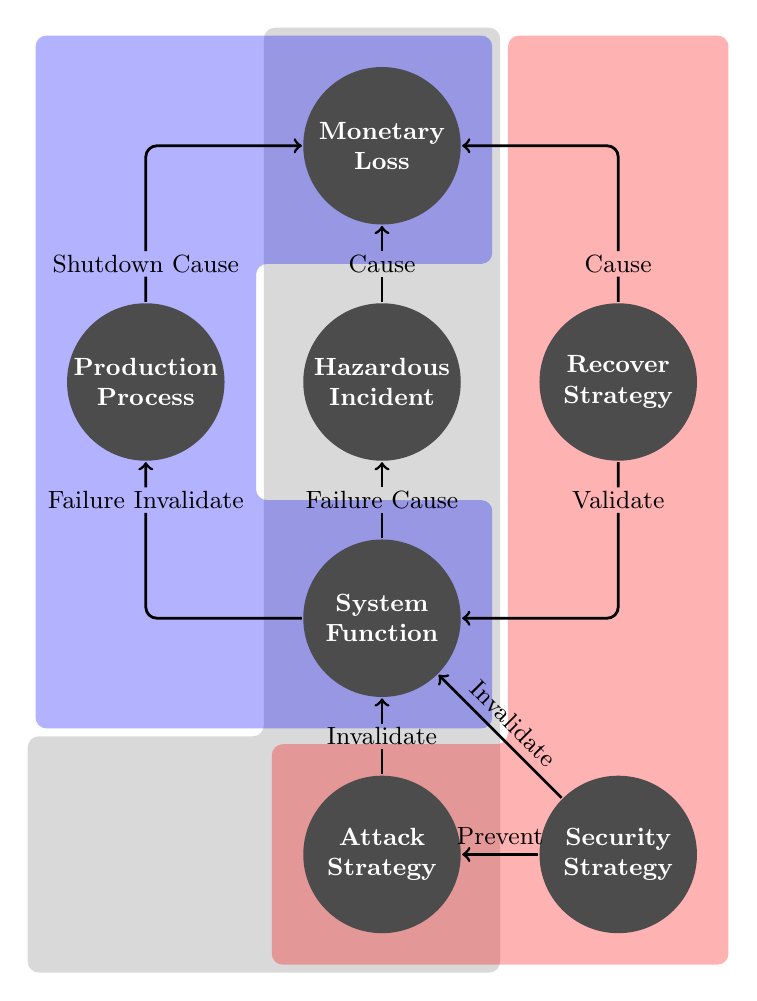
\begin{tikzpicture}[line width = 1pt,
                    factor/.style = {circle, fill = black!70, text = white, font = \bf, inner sep = 0pt, align = center, minimum size = 2cm},
                    tag/.style = {align = center, inner sep = 1pt},
                    model/.style = {rounded corners, opacity= 0.3},
                    arrow/.style = {->, rounded corners}]

\small
\fill[gray, model] (-0.5, 0.5) -- (-0.5, 3.5) -- (2.5, 3.5) -- (2.5, 12.5) -- (5.5,12.5) -- (5.5, 0.5) -- cycle;
\fill[blue, model] (-0.4, 12.4) -- (5.4, 12.4) -- (5.4, 9.5) -- (2.4, 9.5) -- (2.4, 6.5) -- (5.4, 6.5) -- (5.4, 3.6) -- (-0.4, 3.6) -- cycle;
\fill[red, model] (5.6,3.4) -- (5.6, 12.4) -- (8.4,12.4) -- (8.4, 0.6) -- (2.6, 0.6) -- (2.6, 3.4) -- cycle;


\shadowtag[x = 1, y = 2.2]{\bf Multi-level}
\shadowtag[x = 1, y = 1.8]{\bf Bayesian Network}
\shadowtag[x = 1, y = 4.2, color = blue]{\bf Process Model}
\shadowtag[x = 7, y = 4.4, color = red]{\bf Attack-Defense}
\shadowtag[x = 7, y = 4.0, color = red]{\bf Strategies Models}


\node[tag] (AS2SF) at (4, 3.5) {Invalidate};
\node[tag] (SF2HI) at (4, 6.5) {Failure Cause};
\node[tag] (SF2PP) at (1, 6.5) {Failure Invalidate};
\node[tag] (RS2SF) at (7, 6.5) {Validate};

\node[tag] (PP2ML) at (1, 9.5) {Shutdown Cause};
\node[tag] (HI2ML) at (4, 9.5) {Cause};
\node[tag] (RS2ML) at (7, 9.5) {Cause};

\node[factor] (ML) at (4, 11) {Monetary\\Loss};
\node[factor] (HI) at (4,  8) {Hazardous\\Incident};
\node[factor] (SF) at (4,  5) {System\\Function};
\node[factor] (AS) at (4,  2) {Attack\\Strategy};
\node[factor] (PP) at (1,  8) {Production\\Process};
\node[factor] (RS) at (7,  8) {Recover\\Strategy};
\node[factor] (SS) at (7,  2) {Security\\Strategy};

\draw[arrow] (AS) -- (AS2SF) -- (SF);
\draw[arrow] (SF) -- (SF2HI) -- (HI);
\draw[arrow] (HI) -- (HI2ML) -- (ML);
\draw[arrow] (SF) -| (SF2PP) -- (PP);
\draw[arrow] (PP) -- (PP2ML) |- (ML);

\draw[arrow] (RS) -- (RS2ML) |- (ML);
\draw[arrow] (RS) -- (RS2SF) |- (SF);

\draw[arrow] (SS) -- (SF) node[midway, sloped, above] {Invalidate};
\draw[arrow] (SS) -- (AS) node[midway, sloped, above] {Prevent};
\end{tikzpicture}